\section{Implementation}
The following sections describe, how the implementation of the automatic room recognition was achieved. Basically it is split into three parts, later called workflows. Each workflow is a combination of algorithms, which solves a different problem.

Every section will describe why and how the algorithm is implemented and what the results of the implementation was.

\subsection{Workflow 1}
\label{sub:workflow1}
This section describes the first combination of algorithms that was implemented to try and achieve room detection. It is based on research of the paper by Ahmed, Liwicki, Weber and Dengel \citep{mace_valveny_loctea_tabbone_2010} to find the walls in an image with a Hough transformation. To then detect the rooms, the idea was to detect them with a watershed algorithm. This algorithm is used by several projects on the internet, on the context of room segmentation. The general idea, how this algorithm is supposed to work and what problems were found, are described in this section.

\begin{figure}[H]
	\centering
	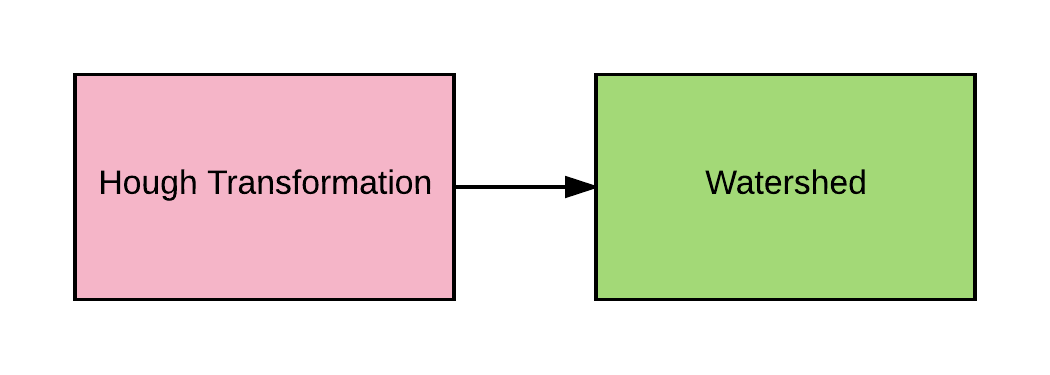
\includegraphics[width=0.8\textwidth]{Workflow1Flowchart}
	\caption{Workflow 1 flowchart.}
	\label{fig:Workflow1Flowchart}
\end{figure}

\subsubsection{Hough transformation}
This implementation is based on the fact that the Hough transformation will find long lines on an image. These lines will usually be the walls. Cleaned up images of architectural floor plans were used to start off. This was done to remove noise on plans and the walls could be extracted easily.

As described in section~\ref{subsubsec:Hough transformation}, the hough transformation finds straight lines on an image. Long straight lines on a floor plan are usually the walls, therefore the Hough transformation is supposed to detect them on the plan. As a precondition for the Hough algorithm, a binary image is needed. To create this binary image, we used the Canny Edge detection algorithm by OpenCV. Wherever it detects an edge, its pixel will be white, all other pixels will be black. There will be two edges for each wall, one where the background changes to the wall and the other, where the wall ends and the background starts again. To then detect the lines, the Hough transformation by OpenCv, called HoughLines, was first used. It finds the all suspected lines and returns it in an array represented with the $(r,\theta)$ orientation representation. The problem with this implementation was, that this just represents the orientation and location of the line but not its size.
As a replacement HoughLinesP was used. It does the exact same, but additionally calculates where those lines actually are. The resulting array returns the actual starting and ending position of the lines. 

\begin{lstlisting}[caption={Hough transformation example code}, label={lst:HoughTransfCode}, language=Kotlin]
//Canny Image
var canny = Mat()
val threshlow = 1.0
val threshhigh = 254.0
Imgproc.Canny(destination, canny, threshlow, threshhigh);

//HoughTransformation
val lines = Mat()
val rho = 1.0
val theta = Math.PI / 180
Imgproc.HoughLinesP(canny, lines, rho, theta, 0)
\end{lstlisting}

The parameters used in the code listing~\ref{lst:HoughTransfCode} are not optimized. Those were chosen as to what worked best with few test runs done on the algorithm. The parameters "threshlow" and "threshhigh" set the threshold for the  hysteresis procedure. The parameter for $\rho$ is set to 1 as a standard, it describes its resolution in pixels. The parameter for $\theta$ describes its resolution in radians.

There were several problems with that algorithm. The algorithm separated a wall line into a lot of small lines. To retrieve the actual wall there would have to be additional computation that connects those several small parts into one big line. As an addition, due to no preprocessing, what was left as a wall, were the actual outlines of the original walls. Therefore any wall was represented by two parallel lines. This would have led to additional effort. Before any of those efforts were made a different algorithm was found that showed more promising results. Therefore the optimization of this algorithm was not pursued further.

  
\subsubsection{Watershed}
The idea to find the different rooms within the floor plan, was to run the watershed algorithm on the image (Section~\ref{subsub:watershed}). It is a flood filling algorithm that starts at given starting points and extends its area, until it meets a wall or a different flood from an other starting point. A further explanation will be done in section~\ref{subsubsub:watershed}, as it was actually implemented and used in our second workflow.

\subsection{Workflow 2}
\label{sub:workflow2}
This section describes the second workflow and what algorithms it is composed of. It is a mix of the work of Sébastien Macé and Peter Dawkins and Hervé Locteau and Salvatore Tabbone~\citep{mace_valveny_loctea_tabbone_2010} and the experiences we made with the first workflow~\ref{{sub:workflow1}}. What it does is, it removes any noise on the floor plan first with morphological operations like erosion and dilation. This is followed up with a room detection algorithm that, in the end, uses the watershed algorithm to determine the rooms. In contrast to the first workflow, where the preprocessing for the watershed was not done sufficiently, this algorithm improved on that. After optimizing this workflow, it was the first workflow that showed actual potential and was able detect the rooms and therefore solve the given problem.


\begin{figure}[H]
	\centering
	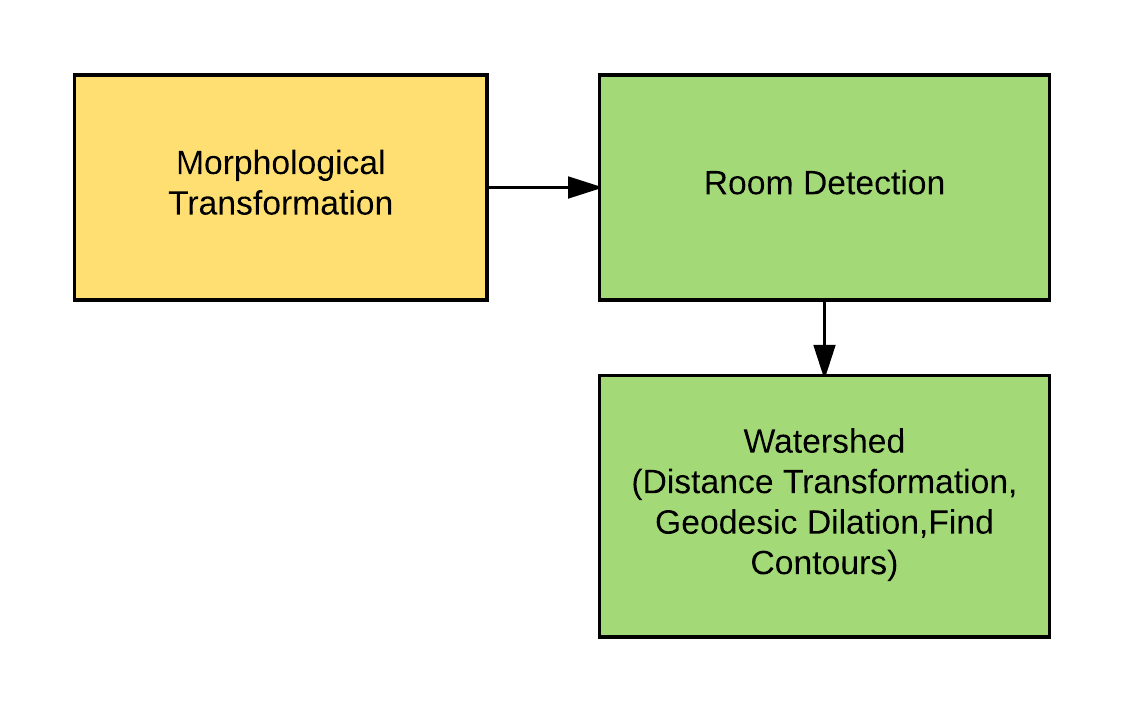
\includegraphics[width=0.8\textwidth]{Workflow2Flowchart}
	\caption{Workflow 2 flowchart.}
	\label{fig:Workflow2Flowchart}
\end{figure}

\subsubsection{Noise removal}
All of the following topics in this section are used to remove or add specific information from our image. The idea is to standardize all incoming floor plans regardless of what "noise" is around in the basic floor plan. Noise is anything that is of no importance to all the following algorithms. This contains elements such as "personal-property" (cars, pianos, etc.) as well as text or any lines to show dimensions on the plan. The idea would be that most of this noise is erased by the user in advance. But it is practically impossible to remove all the noise beforehand due to it being so time intensive that it would ruin all the benefits of the algorithm using less time than doing everything by hand.

\paragraph{Morphological transformation}
\label{sub:MorphologicalTransformation}

The basic principle to remove noise is erosion and dilation. How the algorithm is processed is explained in section~\ref{subsubsec:Erosion and Dilation}.
The purpose of both of those algorithms in this project is to remove any information on the starting picture to get a picture containing only the walls. This works due to the fact that usually the walls are the thickest lines on the floor plan. It is a simple heuristic to extract the walls and is according to the method other papers use. \todo{Link papers}

This project always uses a combination of erosion and dilation to retain the original place of all the walls. The size of the rooms would differ from the original size if we did not do the same dilation after an erosion and vice versa. This would render all the results useless, since a basic requirement is to find the actual room polygon. There are two ways to use noise removal as a combination of erosion and dilation. 

\begin{description}[style=nextline]
	\item[Erosion first] This removes thin lines from the image. Those are non walls and therefore of no importance to the output image. The dilation brings the remaining lines back to its original size.
	\item[Dilation first] This extends all lines and combines any lines that are close to each other. The erosion following then creates one line out of the bunch. This is used to combine walls that are created out of several thin lines into one thick line.
\end{description}

Both of those combinations are used in the morphological transformation class. First used is the "dilation first" transform to combine the walls out of several lines into one. This results in all the walls being one thick line instead of a multitude of small lines. This guarantees that all walls are thick lines and won't get erased with the "erosion first" transform. This is now followed with the "erosion first" transform to erase all the other lines besides the walls. 

\begin{figure}[h]
	\centering
	\subfloat[Original image.]{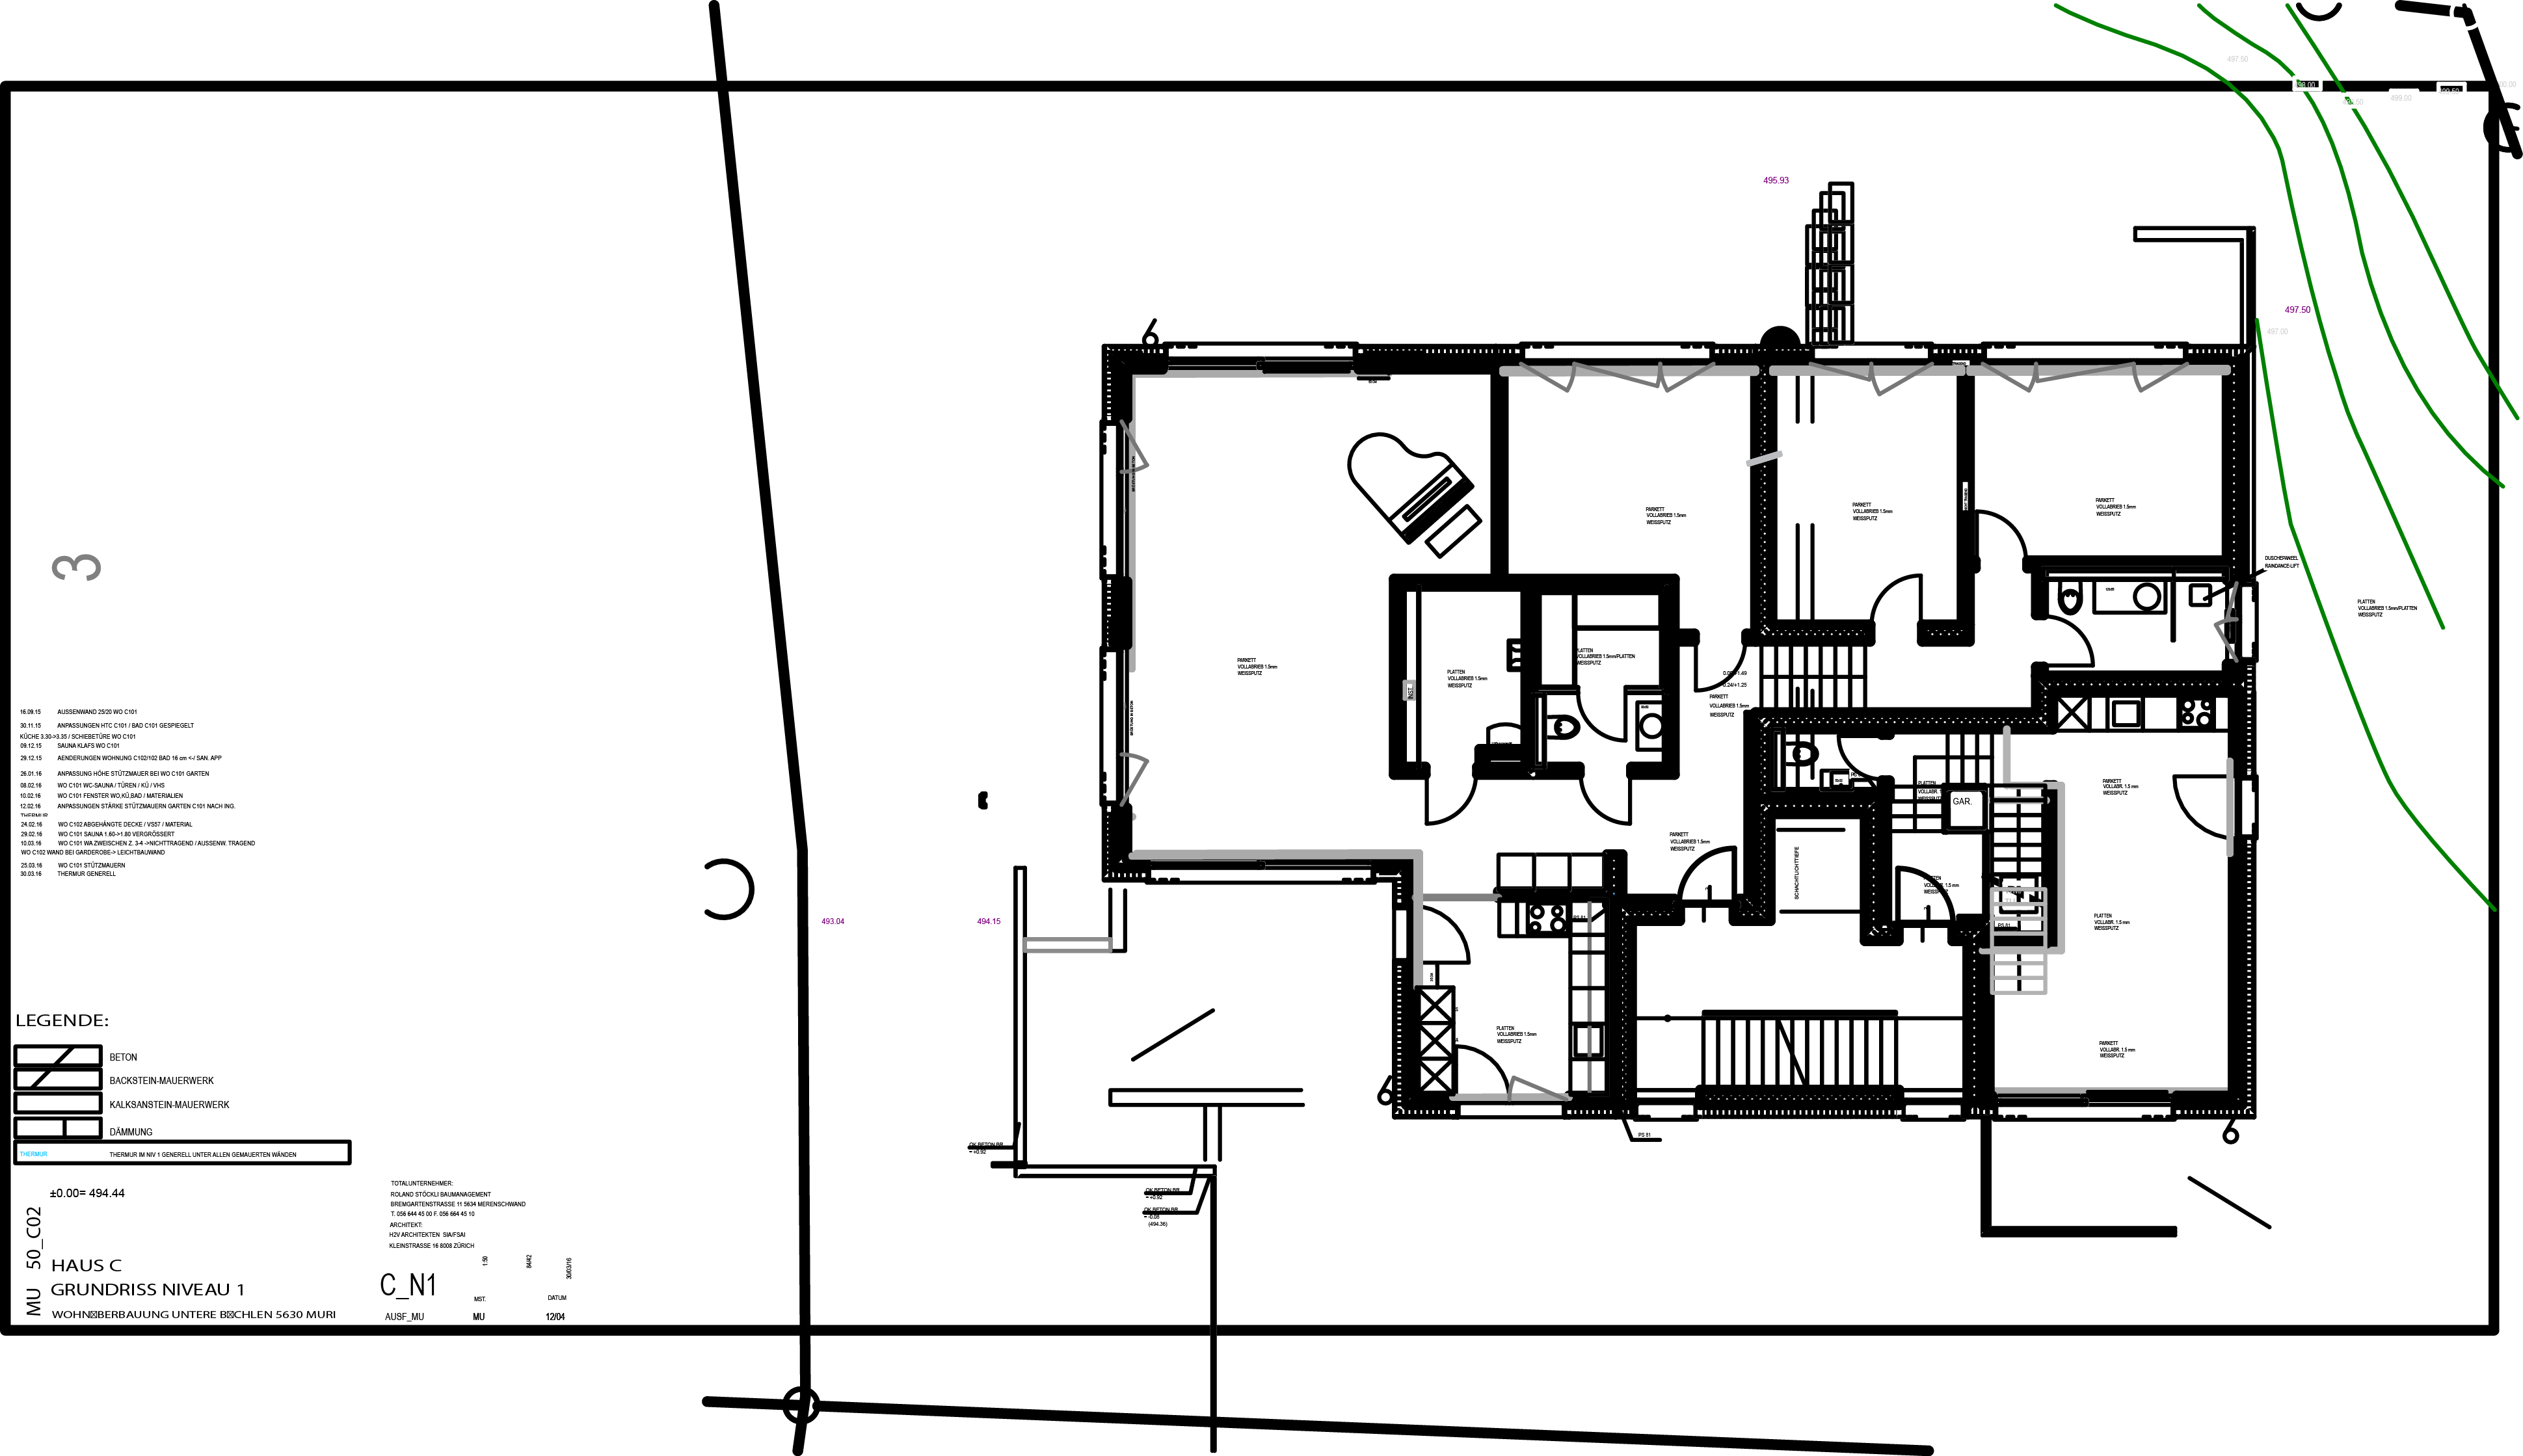
\includegraphics[width=0.5\textwidth]{A_N1.png}\label{fig:A_N1}}
	\hfill
	\subfloat[Image after noise removal.]{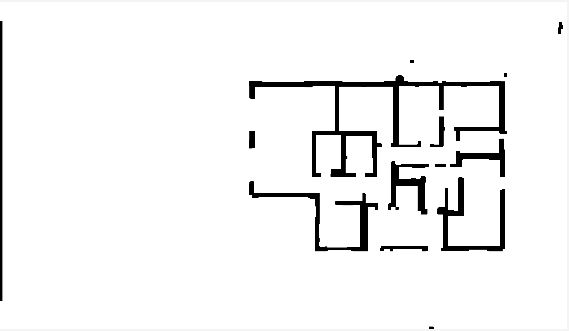
\includegraphics[width=0.4\textwidth]{morphtransuncleaned.jpg}\label{fig:A_N1_Morph}}
	\caption{Before and after of an uncleaned floor plan with noise removal. }
\end{figure}

\begin{figure}[h]
	\centering
	\subfloat[Original image.]{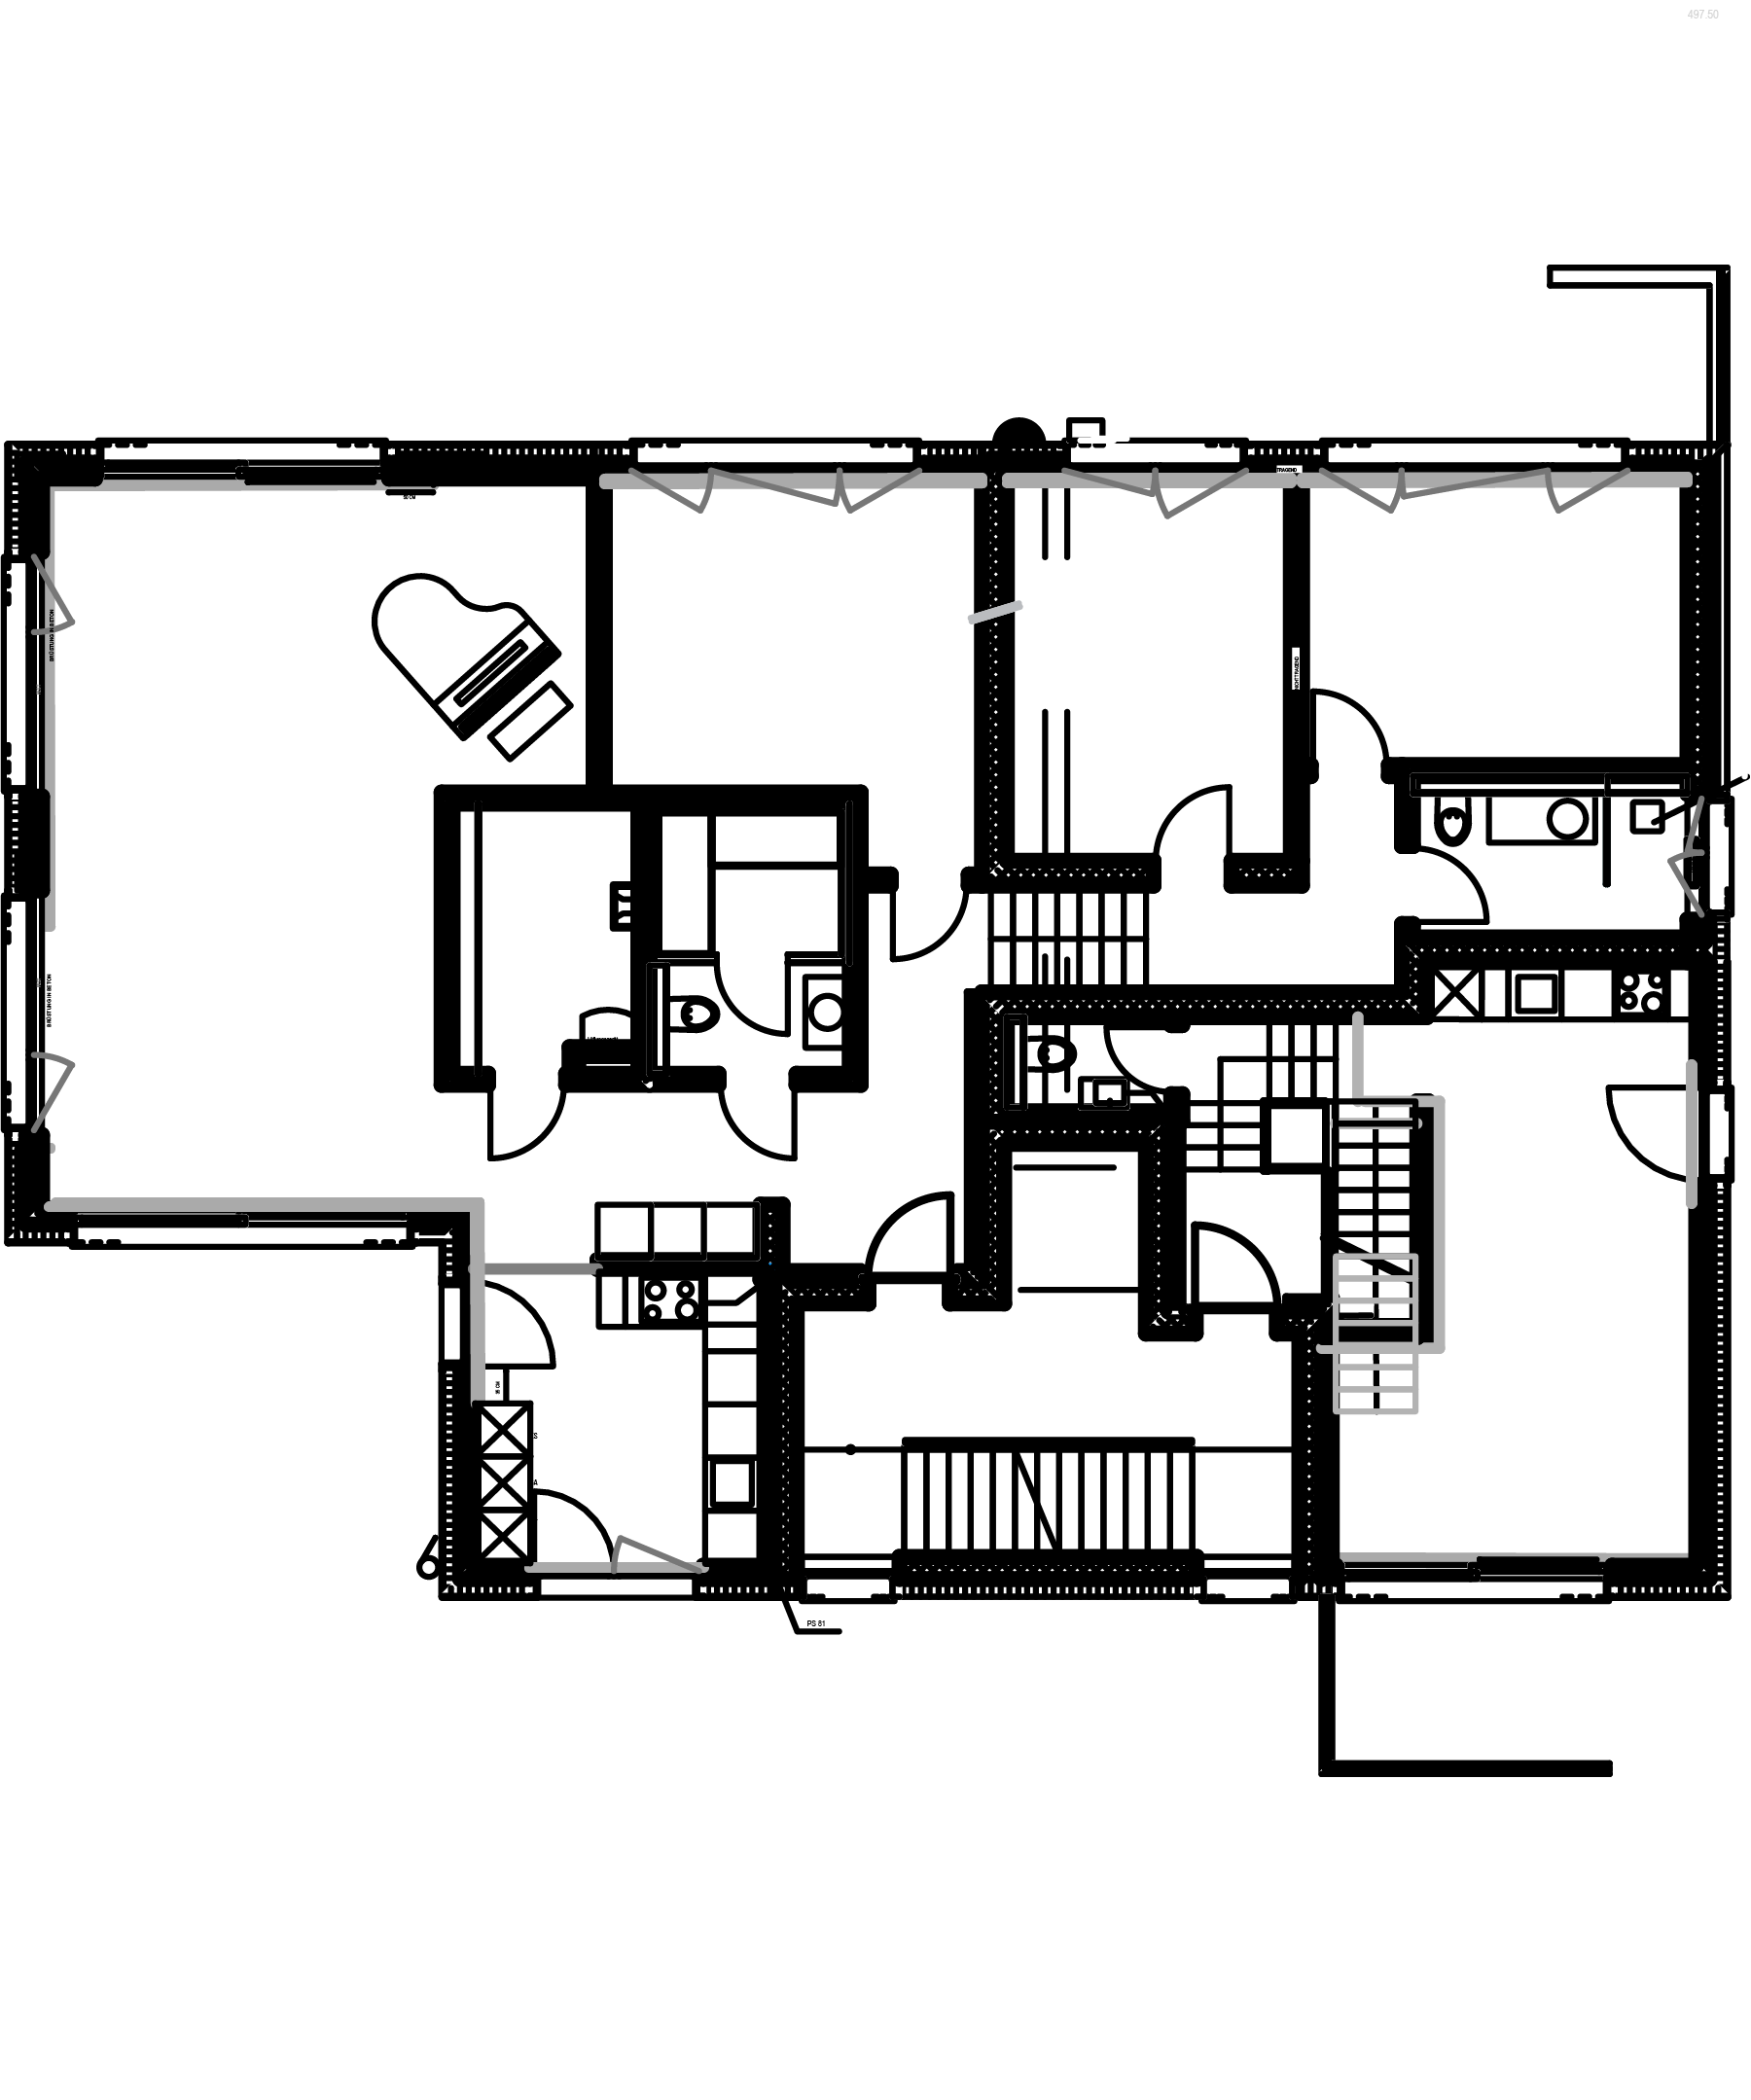
\includegraphics[width=0.5\textwidth]{A_N1_cleaned.png}\label{fig:A_N1_cleaned}}
	\hfill
	\subfloat[Image after noise removal.]{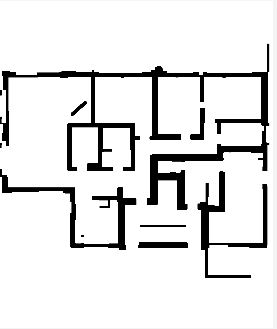
\includegraphics[width=0.4\textwidth]{morphtranscleaned.jpg}\label{fig:A_N1_cleaned_Morph}}
	\caption{Before and after of a cleaned floor plan with noise removal.}
\end{figure}

The figure~\ref{fig:A_N1} is one of the uncleaned testing images before any noise removal. It was cleaned up with an erosion/dilation size of 8. Figure~\ref{fig:A_N1_Morph} is the result of the noise removal. It is easily visible that most of what's left are walls. Due to the thin lines of the windows they get removed in the process. Those will be added later though as they are an important part of the wall to surround the rooms.

The same was done to the cleaned up image. As a result of different image sizes the noise removal was actually worse with the same parameters. This shows that each different image has very specific parameters for an optimal noise removal. This is further discussed in the section \ref{subsec:Parameter Finding}.

As this is not perfect due to the variety of possible objects on a plan, there is the option to delete those beforehand or afterwards with our built in editor. This is so we can manually improve the quality of the outcome of noise removal.

As a result of the noise removal we get an image with very basic information about where the walls are. This will be very important for our next step and other steps to come.


\subsubsection{Room detection}
To implement the room detection, the preprocessing had to be improved compared to the first workflow. What was needed is a proper creation of the foreground and background image. The foreground image contains all the centers of the room. Each center receiving its own color value to differentiate them from each other. The background image contains the all the walls. Those are then combined into a single image and handed over to the watershed algorithm that then finds the rooms. The center of the rooms are found with a combination of a distance transformation~\ref{sub:DistanceTransformation}, a geodesic dilation~\ref{sub:GeodesicDilation} and a contour finding~\ref{sub:FindContours}. All of those are described in the following paragraphs.

\paragraph{Distance transformation}
\label{sub:DistanceTransformation}
The distance transformation is used to find the centers of the rooms as explained in section~\ref{subsubsec:Distance transformation}. As its base it needs a cleaned up image of all the walls. It is a result of the noise removal we discussed in the previous section. To find the actual area of the of the room there is further processing with a geodesic dilation (Section~\ref{subsubsec:GeodesicDilation}) needed.

The distance transformation gives us an image that represents the distance from the walls (lines in black) as a gradient of grey values going from dark (close to the wall) to bright (farther away). This means that there will be a center in each room that is very bright and has color values close to white.

\begin{figure}[H]
	\centering
	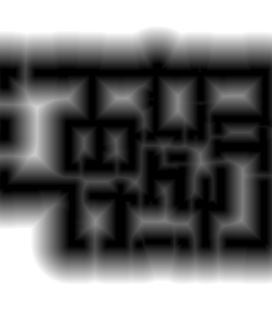
\includegraphics[width=0.8\textwidth]{dist_transform.jpg}
	\caption{Example distance transformation of a architectural floor plan.}
	\label{fig:dist_transform}
\end{figure}

To find the centers there had to be an additional method that provides us with a specific information where these center areas are.
\todo{Discuss specific parameters for each image in parameter finding}
\todo{Distance Transform, Why not Contour Detection}

\paragraph{Geodesic dilation}
\label{sub:GeodesicDilation}
The algorithm to locate the centers after having done the distance transformation is the geodesic dilation~\ref{subsubsec:GeodesicDilation}. The purpose of this algorithm is to find the brightest points in an image and create a marker image. This marker image is a binary image that has all the bright points represented with white color and all other with black color. Based upon the assumption that the distance transformation marked points brighter the further away they are from walls, all room centers consist of bright pixels. Therefore the marker image contains all the room centers. Additionally though, since the plan usually has open space outside the bounding wall, it finds room centers outside of the house as well. The idea was that to close the outside walls and then delete all rooms that are connected to the border of the picture. There is an implementation of this algorithm in workflow 3~\ref{sub:WallClosing}. An implementation of how we tried to avoid this problem is described in the next paragraph about finding contours.

\begin{figure}[H]
	\centering
	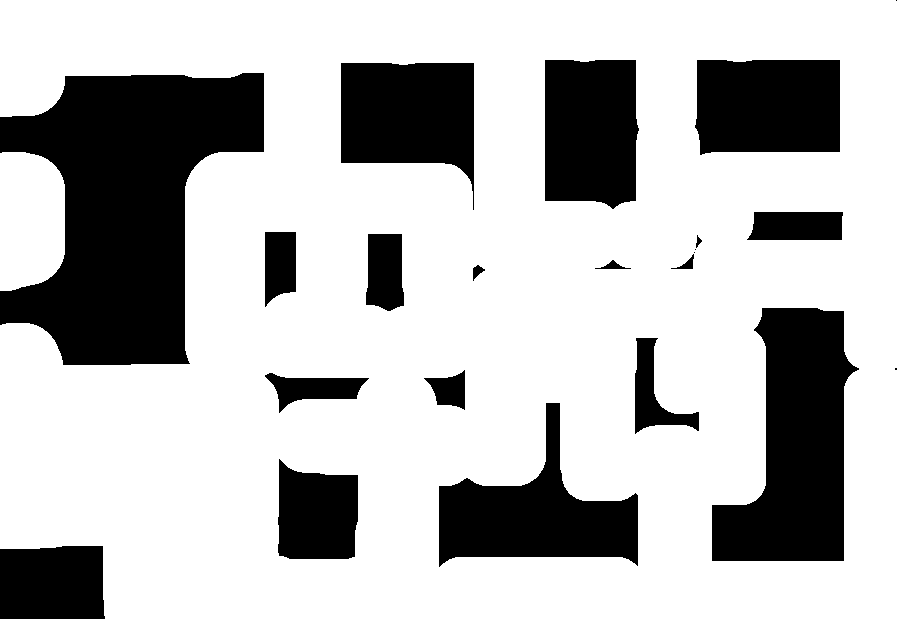
\includegraphics[width=0.8\textwidth]{MarkersGeodesicDilation}
	\caption{This image shows the markers (black areas) for the geodesic dilation of the floor plan AN1.}
	\label{fig:geodesicDilation}
\end{figure}

\paragraph{Find contours}
\label{sub:FindContours}
The find contours algorithm was used to find the centers found in the marker image and give each of those their own color value. This was done so the watershed algorithm automatically creates a border between rooms as soon as the different flooding zones from the algorithm meet each other. This process is further described in the next paragraph. What the find contours algorithm does on the marker image is, that it finds all the borders of the defined centers. With the implementation of findContours in OpenCv you can specify to also fill the found borders with a specified color value. Therefore each marker found got a new color value. As it is a grayscale image, a base value of 200 was defined and for each new room found we increased that color for that room by one. This gives the option the detect up to around 50 rooms.

\begin{figure}[H]
	\centering
	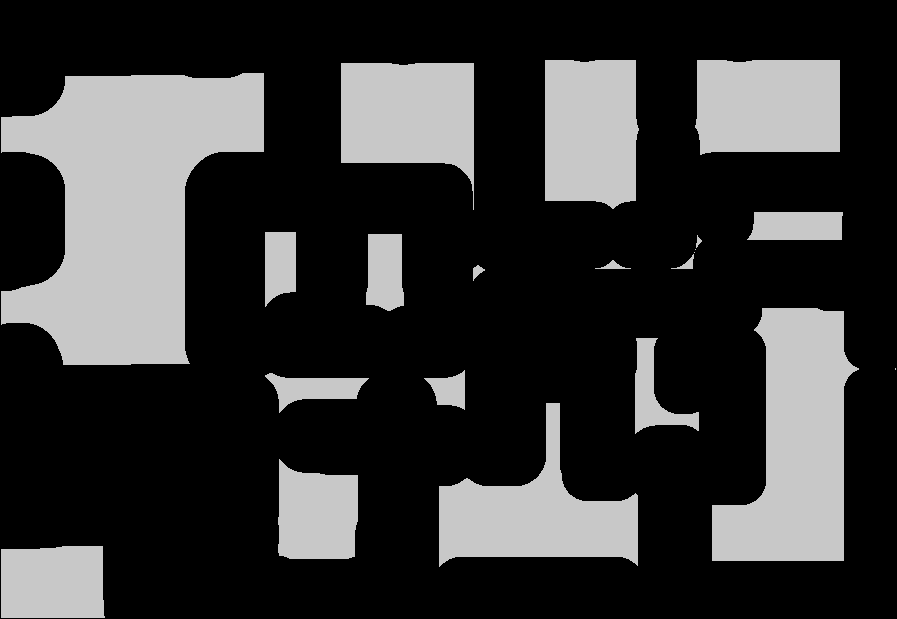
\includegraphics[width=0.8\textwidth]{findContourForeground}
	\caption{This image shows the different marker centers colored in pixel values around 200 and higher on the plan AN1.}
	\label{fig:findContour}
\end{figure}

An additional idea that was tried was to ignore rooms found that had any connection to the border of the image. The findContours algorithm finds a hierarchy on what contour contains other contours. We therefore tried to use the heuristic that the out-most contour that contains all other contours is the contour that contains all "room-centers" that are outside of the house. Therefore this contour could be ignored. As you can see on the image \ref{fig:geodesicDilation}, this heuristic does not work very well as there are to many conditions that can make it fail. One problem was that windows weren't closed and actual room centers existed that connected to the wall itself and therefore were not an inner contour. Additionally there are sometimes inner contours that are not part of the house itself. As a result of those experiments we came up with a solution that is described in workflow three as wall closing~\ref{sub:WallClosing}.

 
\paragraph{Watershed}
\label{subsubsub:watershed}

The watershed is the core of our room search algorithm. Its purpose is to fill  the unknown areas that are provided in a foreground/background image from previous images. It needs extremely good preprocessing. If it has any previous errors, the resulting rooms will not make sense.

We use the watershed to its ability to find connected rooms with a simple method. It is a simple algorithm that has low computational cost. This and the fact that it was already implemented in openCV makes us use this algorithm.

The algorithm uses a simple image of all the walls as an image to compare to the foreground/background image. This image has been modified with the door recognition algorithm to close all doors within that picture. This is important so rooms are separated when running the watershed algorithm. Additionally we tried to do a window recognition to close the outside walls. As explained in section \todo{Explain why window rec didnt work}, this did not work out as planned. What we instead used was \todo{create alternative to window recognition}. With this method we are able to separate all rooms within a building that has no windows on the inside. Any building that has a courtyard will fail with this method. Our goal was to find a solution that can also deal with this. But due to limited time and no reasonable alternative we chose to go with that.

The background/foreground image is split up in three different zones. The zone with pixel color values of 0 represent the part of the image that are unknown. All pixels with color value \todo{findValue} represent the walls. As for the rooms we chose to mark all center with value \todo{findValue}. The image used for comparison has the same areas with walls as the BG-image. This means that the area for the wall will not expand with the watershed. The only exception is the area where doors or windows were closed. This is based on the assumption that the wall has the same pixel color and the inside of the room has a vastly brighter color.
The bright centers of the room inside the BG-image will expand into the unknown areas close to the walls and fill up the rooms. This will result in an image with several enclosed rooms all having the same pixel color. This will be processed with a modified connected components algorithm to find all the edges or the room.

We ran into several problems during the implementation of this algorithm. The most common problem is that not all doors were found. Additionally not all rooms have doors to separate them. There are also rooms that are separated with just an open space. There are also objects like cabinets that were drawn with thick lines and were identified as a part of the room. This is easily recognizable as a human but can not be differentiated with the algorithms used.

As a solution to the fact that not all the doors are found, there is the option to close doors by hand with the editor. This is the simplest solution that always guarantees success. We also tried to improve door detection with better samples and bigger sample size. This can be found in the section \todo{link section with door detection}.
To erase object from the image we initially planned to do an object detection. There was time to do some additional object detection other than just door and window. Those can be found in the code. But there are too many different object only within those few plans we got to catch them all. To implement all of the and erase those objects is a next step for this project. For now the user has to erase all object that do not get caught by noise removal by hand.
\todo{Watershed}


\subsection{Workflow 3}
\label{sub:workflow3}
With all the gained experience in workflow one (Section~\ref{sub:workflow1}) and workflow two (Section~\ref{sub:workflow2}), we started to implement workflow three. This workflow improves the room detection with the use of object detection, to fill gaps caused by the morphological transformation (Section~\ref{sub:MorphologicalTransformation}).

\begin{figure}[H]
	\centering
	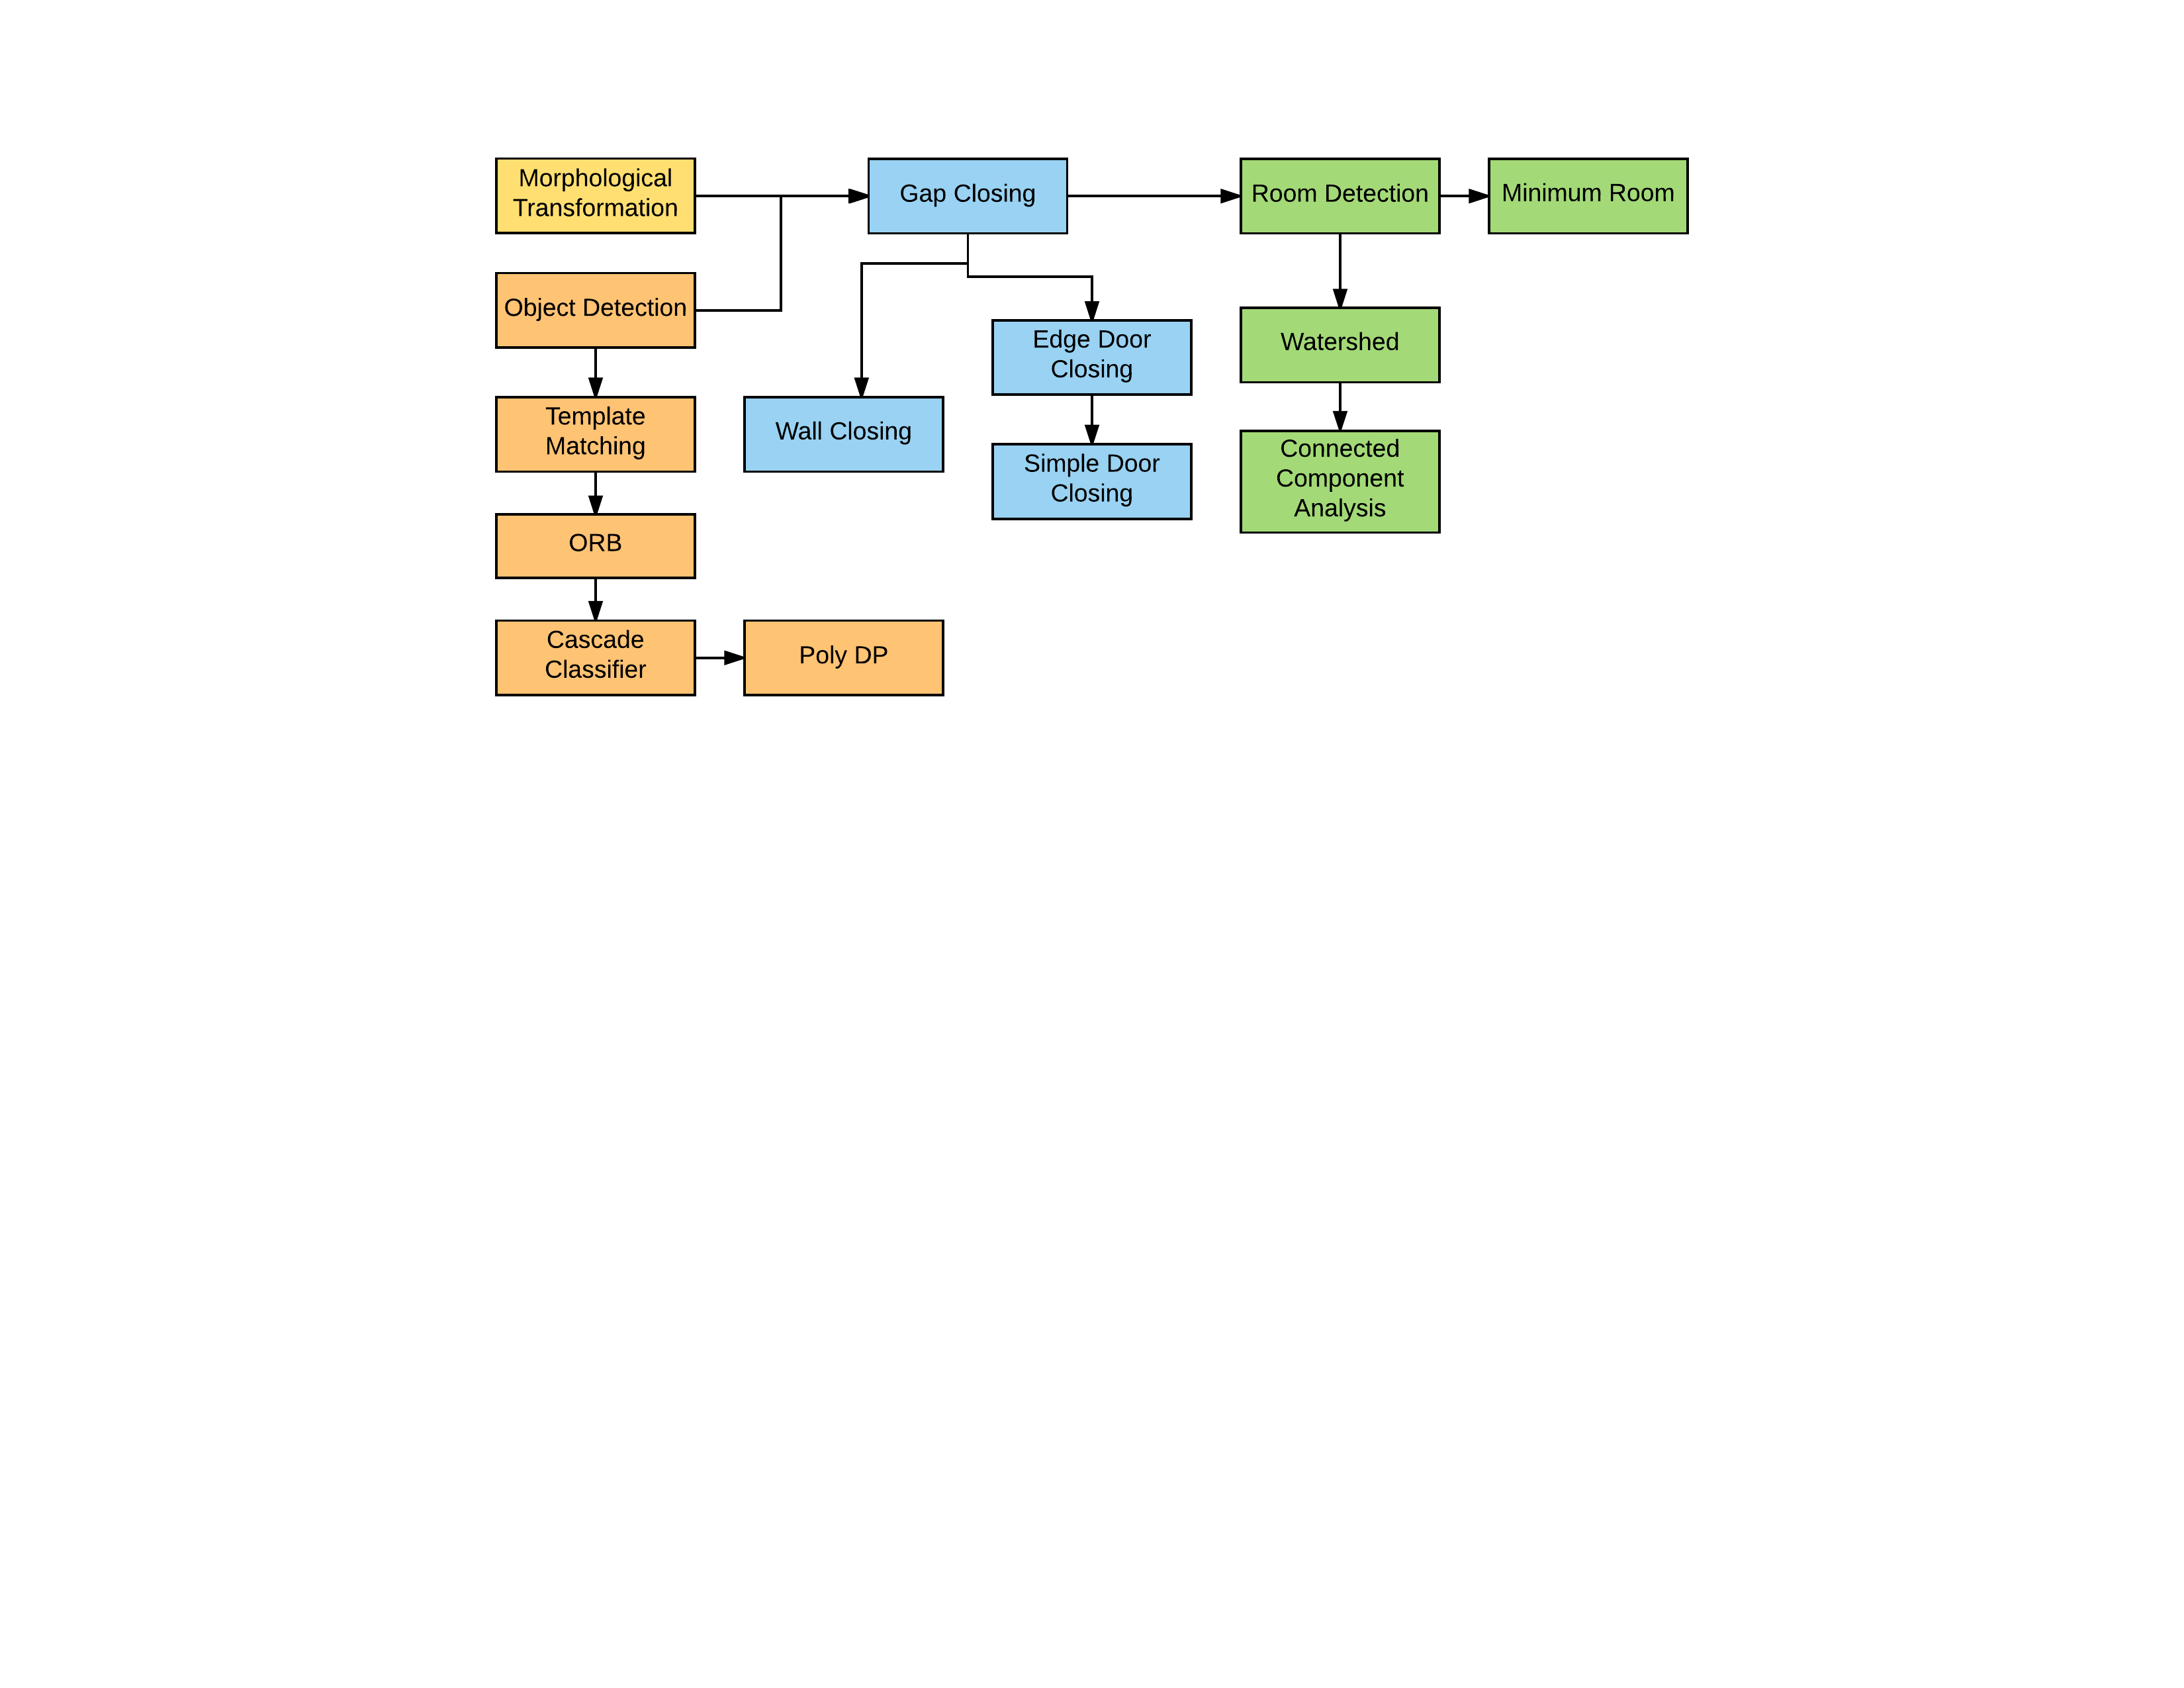
\includegraphics[width=1.0\textwidth]{Workflow3Flowchart}
	\caption{Workflow 3 flowchart.}
	\label{fig:Workflow3Flowchart}
\end{figure}

As shown on figure~\ref{fig:Workflow3Flowchart}, the morphological transformation and object detection step can be run in parallel. Because the user interface needs the assistance of the user, we decided to first run the object detection and then run the morphological transformation.

\subsubsection{Noise removal}
Noise removal has not been changed from the previews workflow. Morphological transformation is still used in this workflow, to detect the inner and outer walls of the building and to remove unwanted noise from the image like furniture or architectural markings.

For more information about the noise removal, have a look at section~\ref{sub:MorphologicalTransformation}.

\subsubsection{Object detection}
One of the major problems of workflow two (Section~\ref{sub:workflow2}) is, that the morphological transformation erases too many elements from the floor plan. The doors and windows are also removed, but they are needed to separate the individual rooms.

Object detection was contemplated from the beginning of the project, to detect furnishings and other parts of a room, which define the room zones (Section~\ref{sub:RoomZones}). So the idea was to use it, to detect doors and windows and solve the problem of workflow two.

There are many 

\paragraph{Template matching}
\paragraph{ORB}

\todo{JavaCV}
Hough line transformation was the first algorithm we tried using to find the walls in the floor plan. It finds straight lines  

\paragraph{Poly DP}
\paragraph{Cascade classifier}
The cascade classifier is used for object recognition of doors, windows and other objects that are important for the room detection and zone identification. This algorithm is a machine learning algorithm that has to be trained with positive and negative images. The resulting learned parameters are saved in an XML file. Since this is a crucial part of this project, it is described more detailed than most other algorithms. In the following lines the implementation process is described as well as all the experiences we made during this project.

The basic problem was to find an algorithm that can find objects that vary in their details and regardless of their rotation and size. This is important due to the fact that there is no standard for objects in architectural floor plans that are used by a wide audience of architects. The decision to go with a machine learning approach and not an algorithm that works with heuristics is because we wanted to be able to process a broad variety of floor plans. Regardless whether they show a small house with just basic features or a big plan with a lot of details and special objects.

\subsubsection{Gap closing}
\paragraph{Edge door closing}
\paragraph{Simple door closing}
\paragraph{Wall closing}
\label{sub:WallClosing}
\subsubsection{Room detection}
\paragraph{Watershed improvements}
\paragraph{Connected components}
\paragraph{Minimum room deletion}


\todo{subsubsubsections for further titles?}